\subsection{Übersicht}
\label{subsec:Uebersicht}
Um eine bessere Vorstellung über die Wetterstation zu erhalten, wird hier das noch unbestückte PCB grafisch dargestellt und die verschiedenen Komponenten erläutert. Um die Übersichtlichkeit wahren zu können, werden in verschiedenen Bildern die Hauptbereiche mit einem roten Rahmen markiert und mit einer Zahl, jeweils neu beginnend bei 1, versehen. Wichtige Teilbereiche werden ebenfalls markiert und mit einem Buchstaben versehen, jeweils neu beginnend bei A.

\begin{figure}[h]
\centering
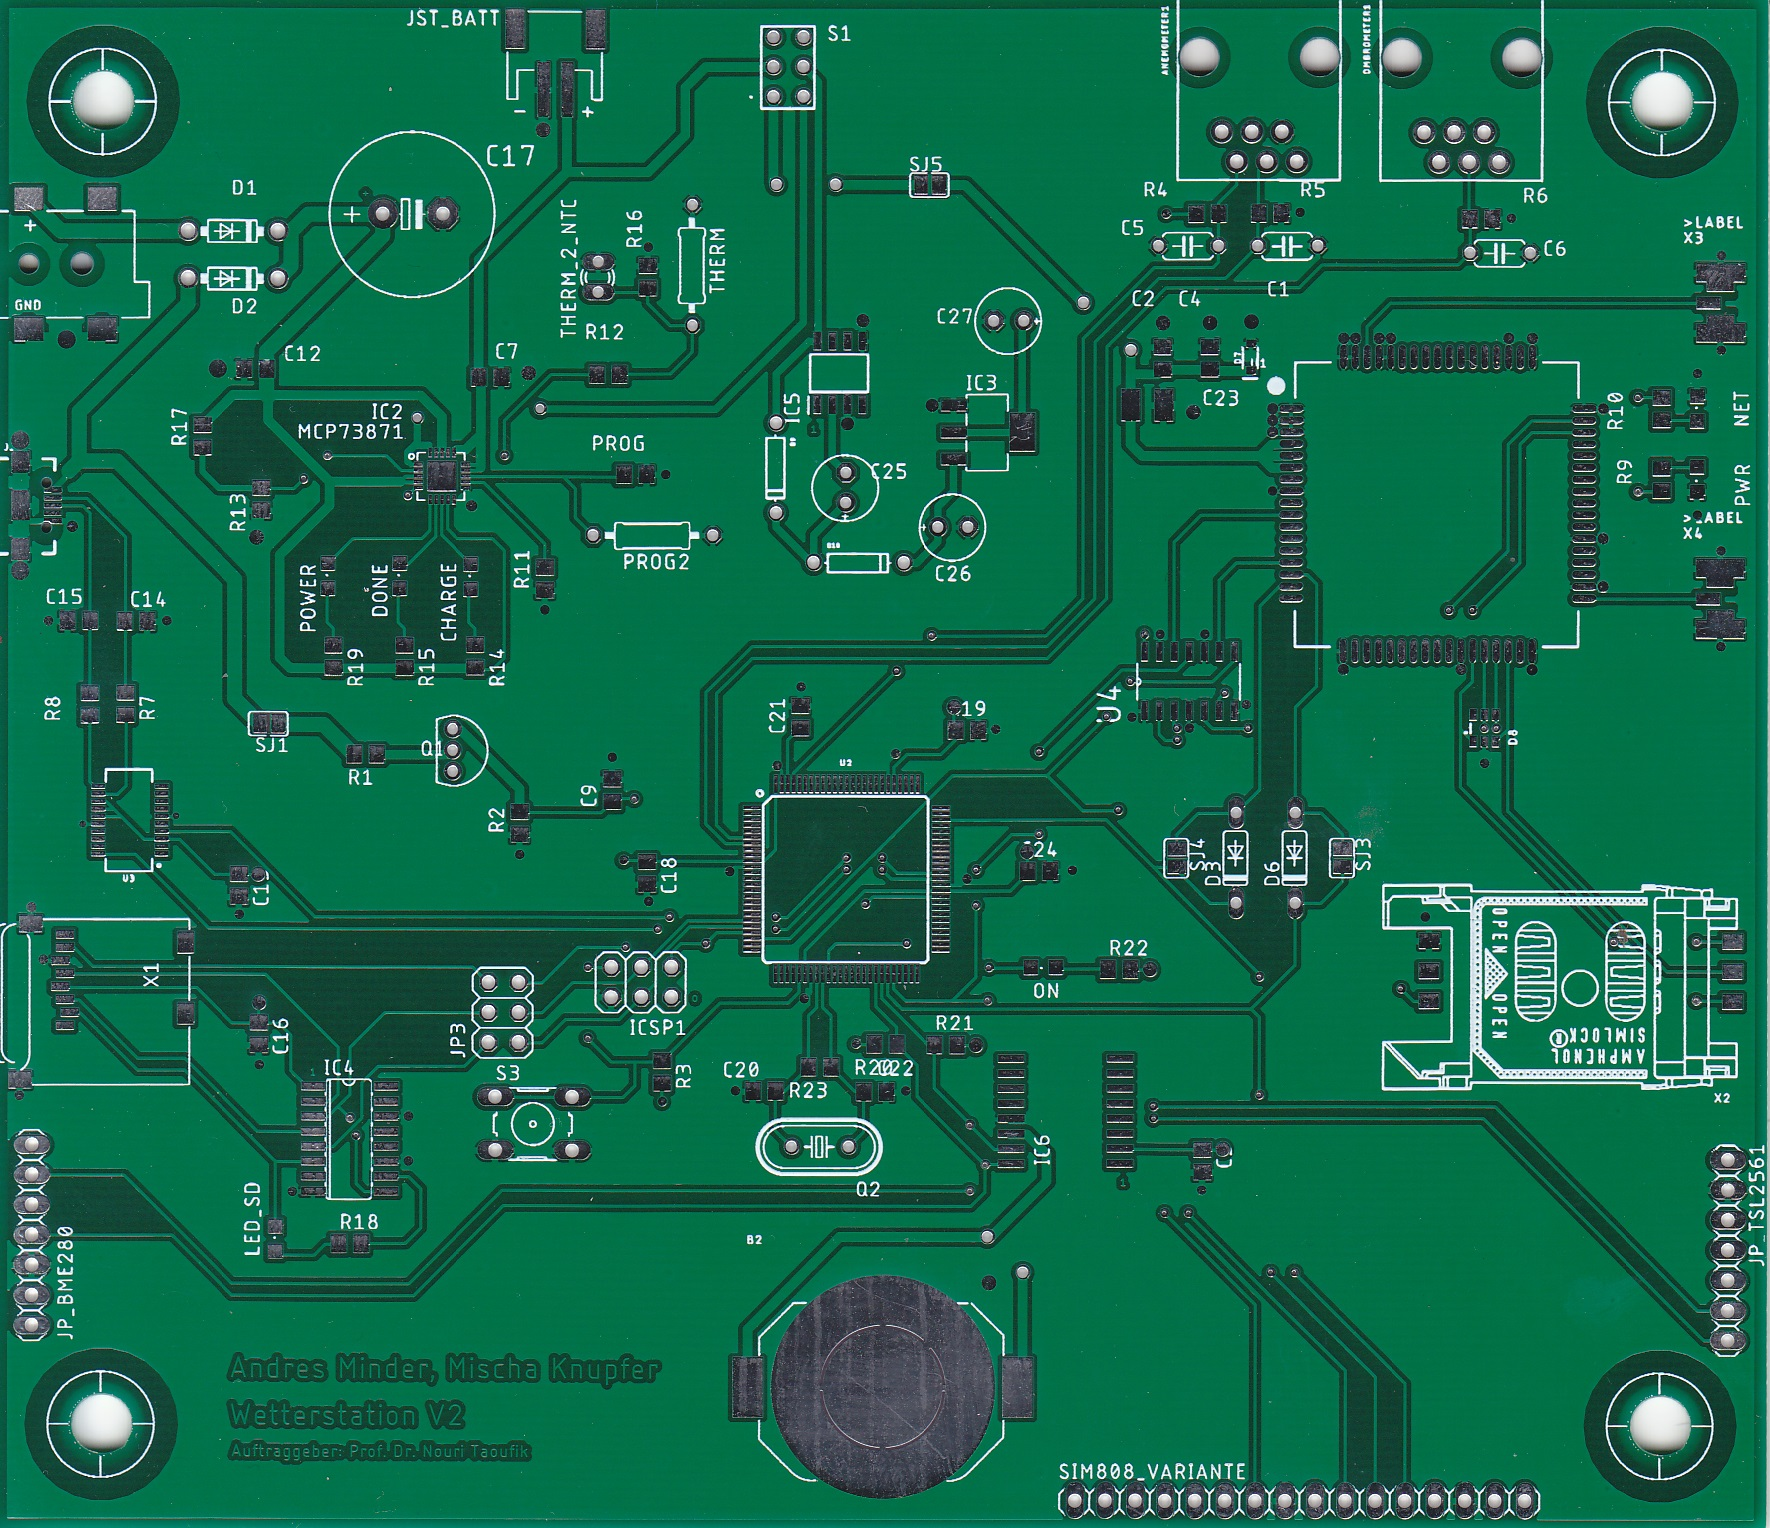
\includegraphics[width=0.99\linewidth]{graphics/HW_Uebersicht/PCB_Unbestueckt.jpg}
\caption{Das noch unbestückte PCB.}
\label{fig:Uebersicht_PCB_blank}
\end{figure}
Abbildung \ref{fig:Uebersicht_PCB_blank} zeigt das noch unbestückte PCB ohne markierte Bereiche. Man erkennt deutlich die Leiterbahnen sowie die Lötpads für die verschiedenen Bauteile. Welche Bauteile nun zur gleichen Bauteilgruppe gehören wird mit den nächsten Abbildungen erkenntlich.

\newpage

\begin{figure}[h]
\centering
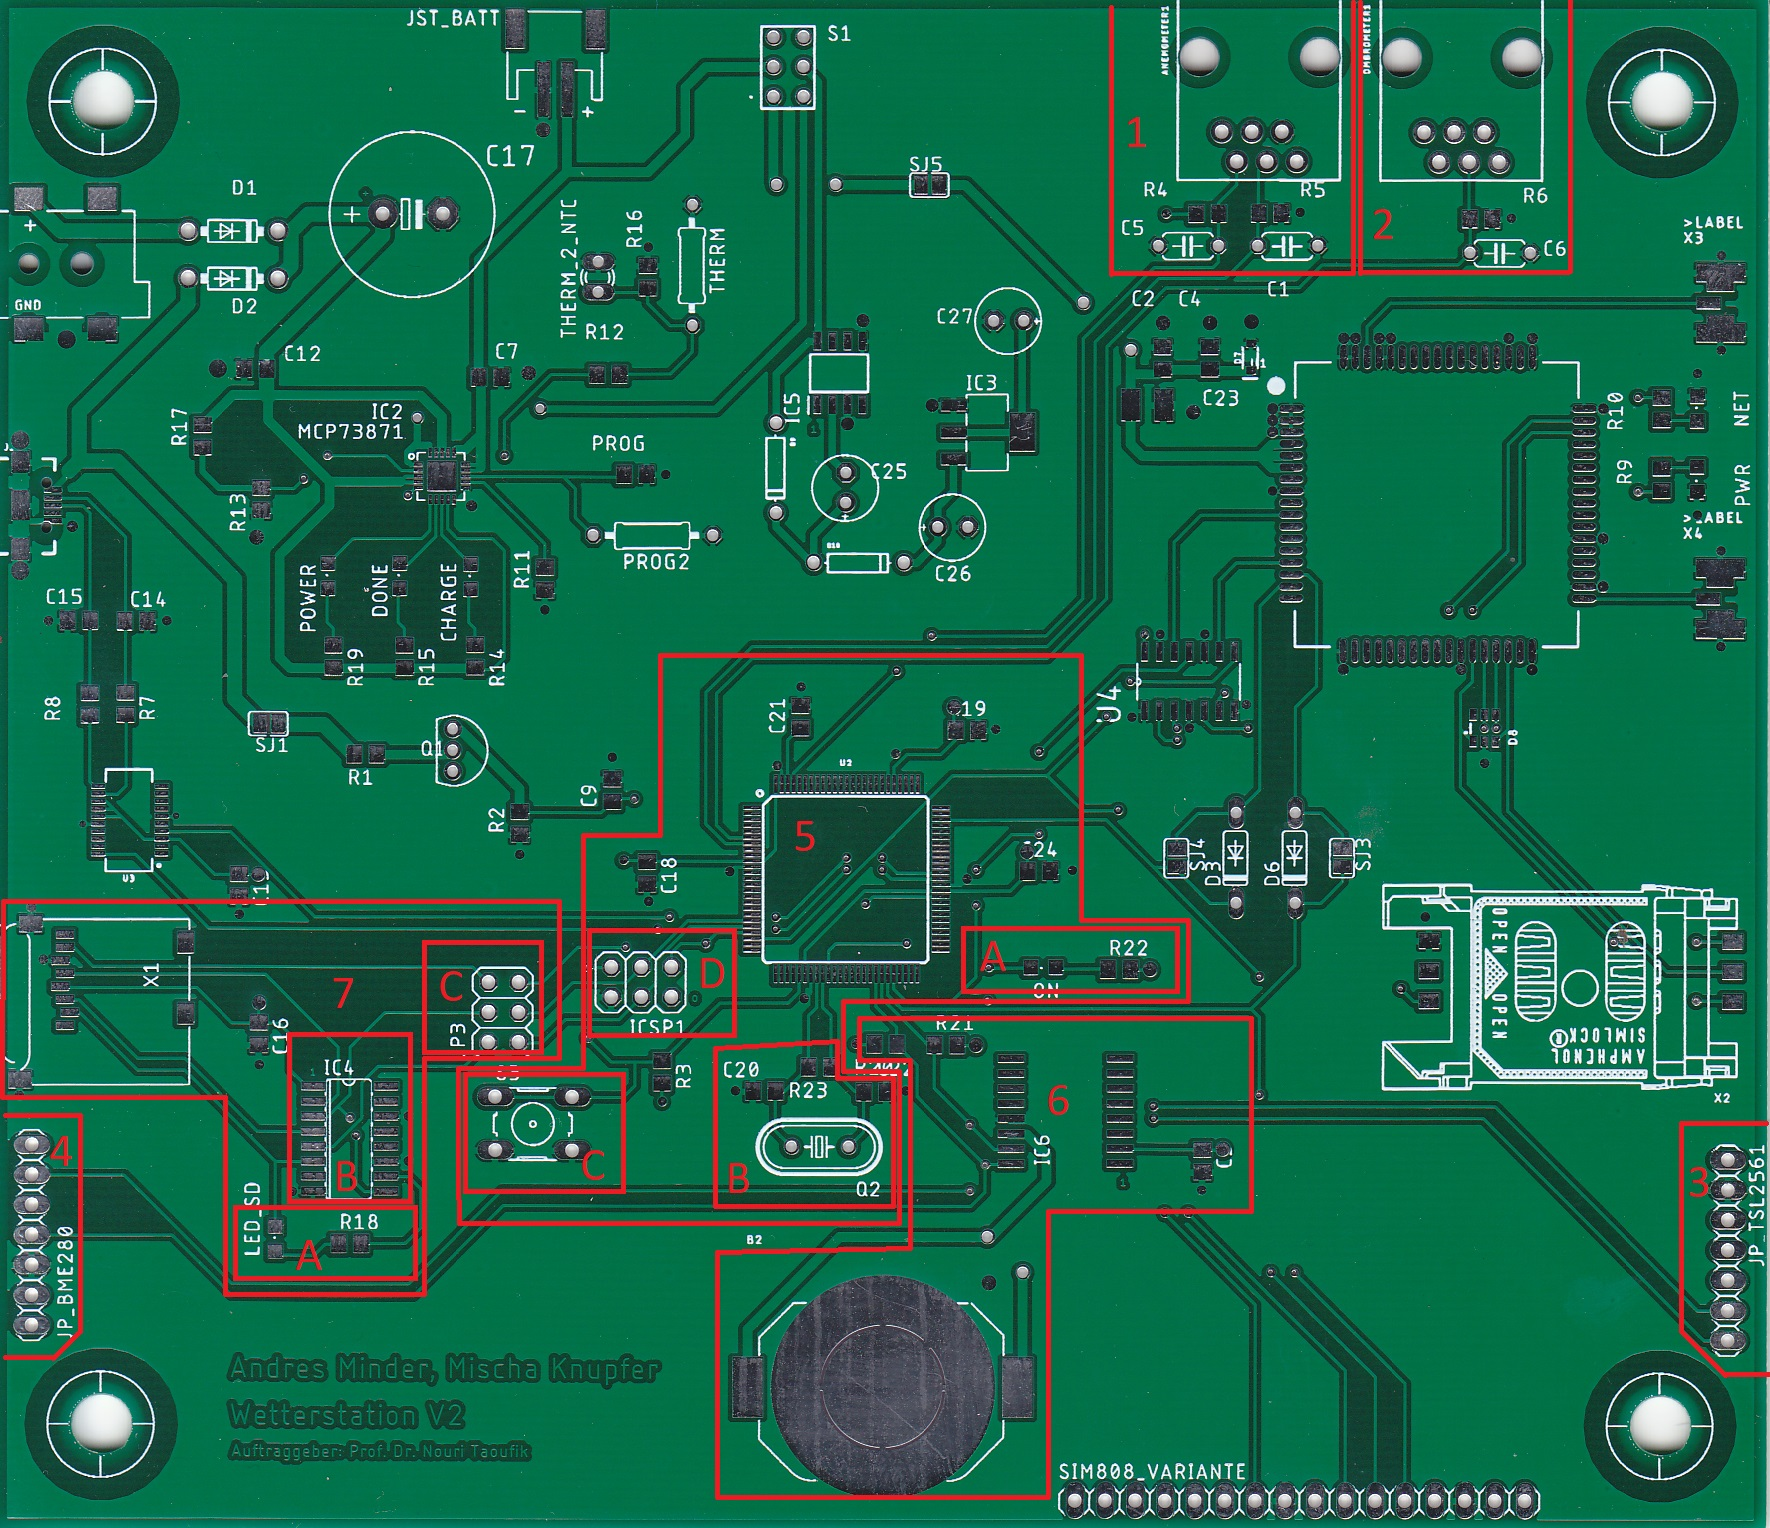
\includegraphics[width=0.99\linewidth]{graphics/HW_Uebersicht/PCB_Sensoren_MCU_SD_RTC.jpg}
\caption{Das unbestückte PCB mit den markierten Bereichen der MCU, der Datenspeicherung, der RTC und der Sensoren.}
\label{fig:Uebersicht_PCB_MCU_RTC_SD_Sense}
\end{figure}
Sieben Bauteilgruppen wurden in der Abbildung \ref{fig:Uebersicht_PCB_MCU_RTC_SD_Sense} markiert. Markierung 1 zeigt den RJ11-Stecker für das Anemometer mit Windrichtungsgeber, wobei an den Ausgängen jeweils ein RC-Filter angefügt wurde um Störungen im höheren Frequenzbereich herauszufiltern, um so ein nutzbares Signal zu erhalten. Das Ombrometer trägt die Markierung 2 und besitzt ebenfalls ein RC-Filter am Ausgang. Die 3 markiert die Pinleiste für den Anschluss des TSL2561 (Lichtintensitätssensor), ein nach aussen geführtes Breakout Board. Gleich Verhält es sich mit der 4, dem BME280. Die 5 markiert die Bauteilgruppe der MCU (ATMega2560), welche 4 wichtige Untergruppen beherbergt. 5-A zeigt eine Status-LED, welche leuchtet, sobald die MCU in betrieb ist. 5-B ist ein externer Clock, welcher der MCU den Takt vorgibt. Ein Reset der MCU und somit des Systems ist über den Reset-Button (5-C) möglich. Über 5-D, ein ICSP-Header (In Circuit System Programming), kann die MCU mit der Firmware geladen werden. Die 6 markiert die Bauteilgruppe des RTC (Real Time Clock) mit der zugehörigen Stützbatterie (CR2032 Knopfbatterie). Die 7-te Bauteilgruppe ist die Datenspeicherung. 7-A zeigt ein Status-LED, welche bei Aktionen mit der $\mu$SD-Karte aufleuchtet. 7-B beherbergt ein IC mit integrierten Operationsverstärkern, welche die Leitungen der $\mu$SD-Karte treiben. Über 5-C kann die Datenspeicherung über Jumper abgekoppelt werden, dies ist notwendig, da es während des Ladens der Firmware auf die MCU es sonst zu unkontrollierte Zugriffe auf die $\mu$SD-Karte kommen kann.

\begin{figure}[h]
\centering
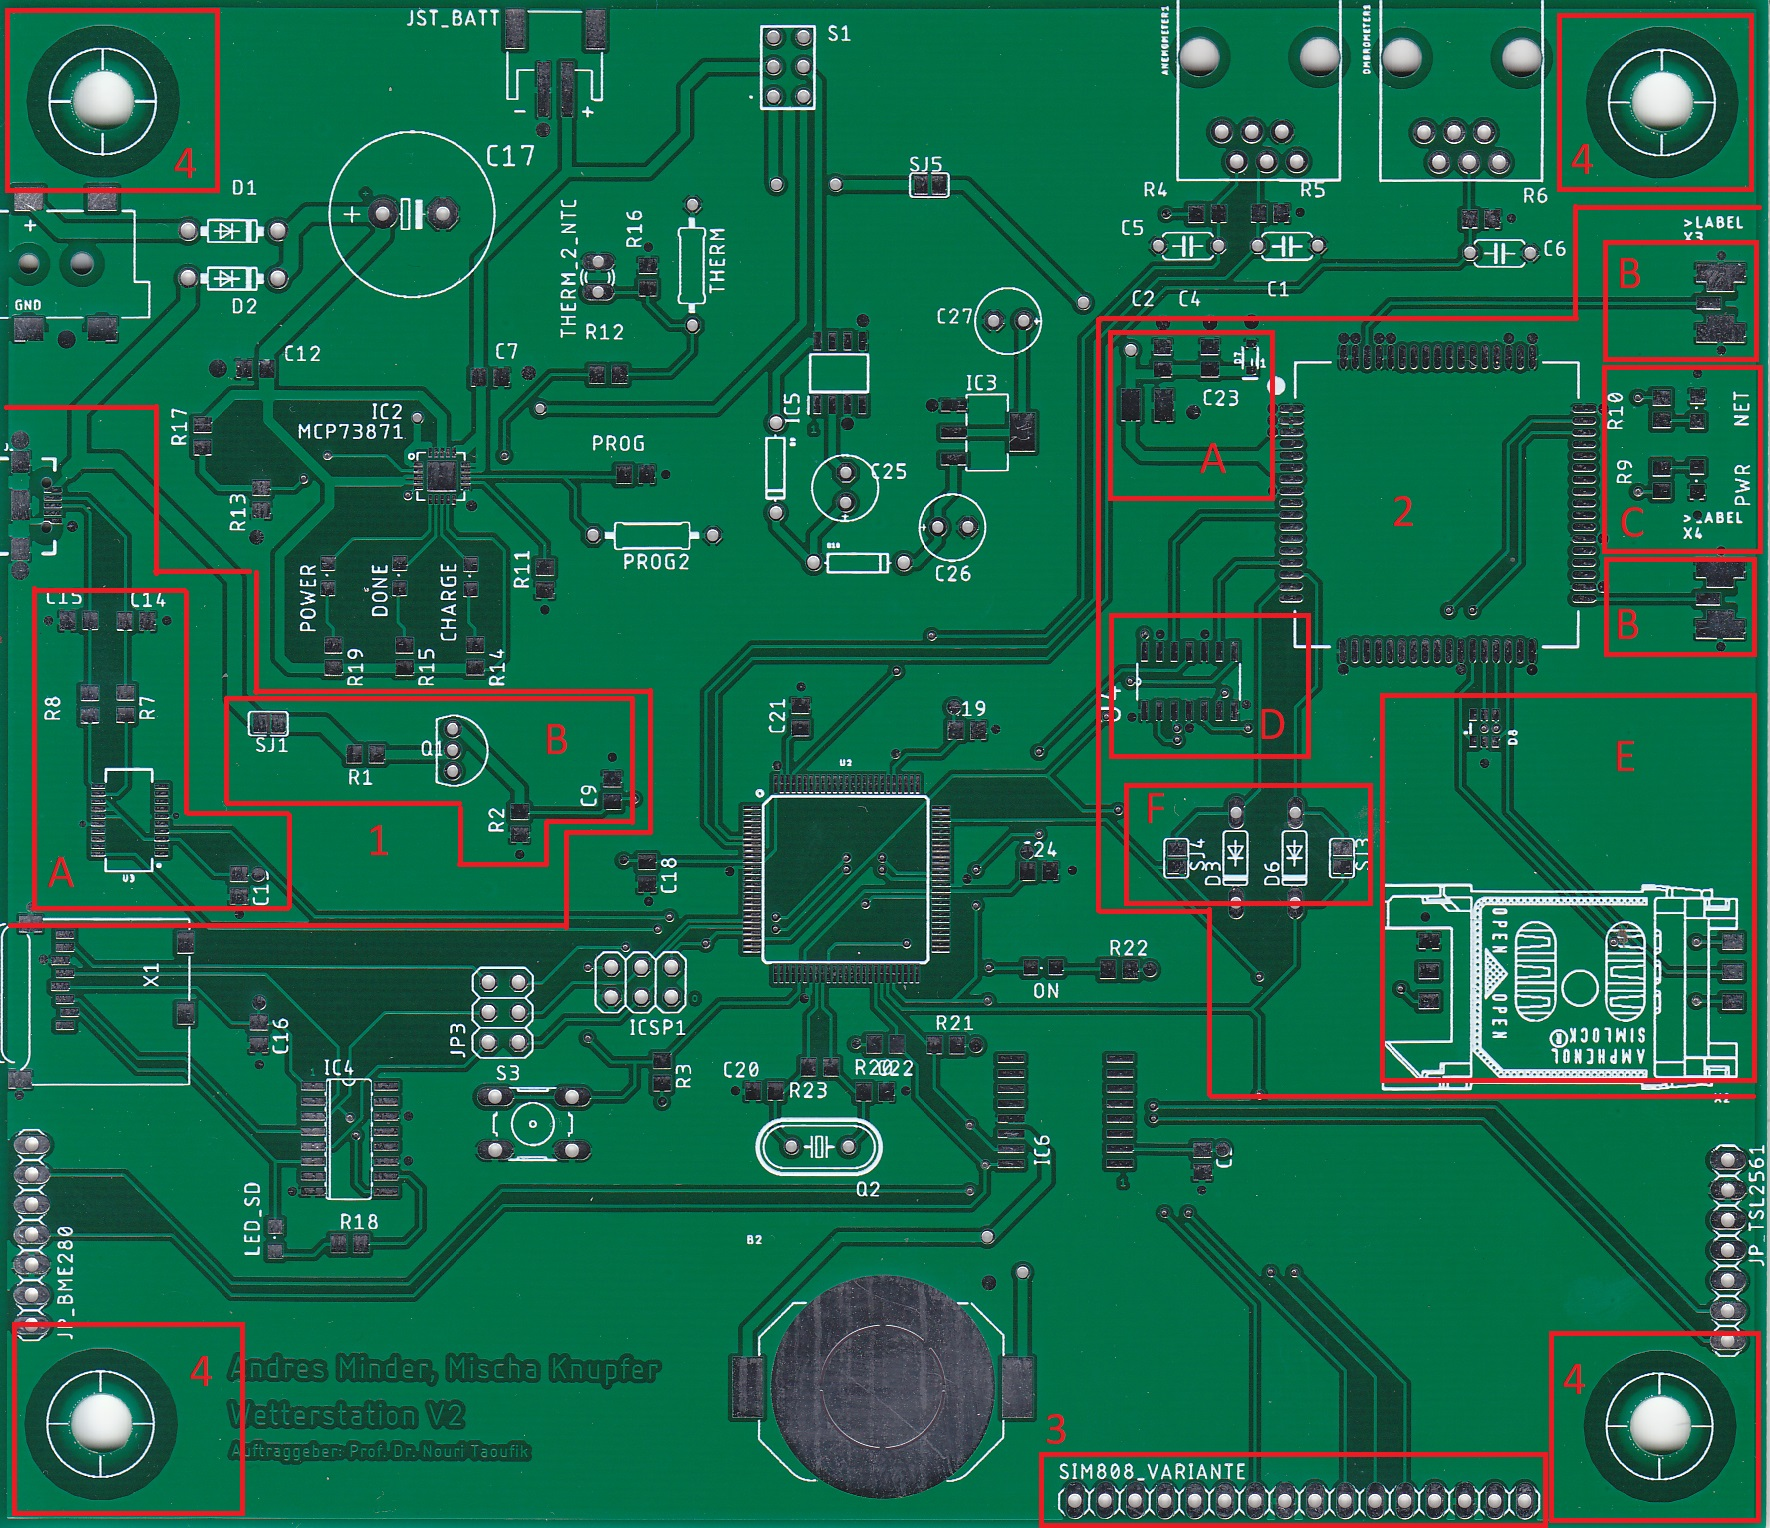
\includegraphics[width=0.99\linewidth]{graphics/HW_Uebersicht/PCB_USB_SIM808.jpg}
\caption{Das unbestückte PCB mit den markierten Bereichen des $\mu$USB-Interfaces, des SIM808 und der Bohrlöcher für die Montage im Gehäuse.}
\label{fig:Uebersicht_PCB_USB_SIM}
\end{figure}
Abbildung \ref{fig:Uebersicht_PCB_USB_SIM} zeigt die markierten Bereiche für die SIM808 (2), des $\mu$USB-Interfaces (1) und die Bohrlöcher für die Montage des PCBs im Gehäuse (4). Ausserdem gibt es eine Bestückungsvariante (3), bei der ein Breakout Board des SIM808 angeschlossen werden könnte, falls die On-Board Variante nicht funktionieren sollte. Im Bereich des $\mu$USB-Interfaces (1) sieht man deutlich zwei Teilbereiche, A und B. Teilbereich 1-A enthält den FT231XS, ein USB-to-UART IC, und dessen Beschaltung gemäss Datenblatt \cite{FTDI}. Für die Anschlusserkennung wird die Schaltung im Teilbereich 1-B verwendet. Für die SIM808 wird eine SIM-Karte (2-E) verwendet, sowie Antennen (2-C) und eine Schaltung zur Stabilisierung und Entstörung der Speisung (2-A) benötigt. 2-C beinhaltet zwei Status-LED, um den Betrieb und die Konnektivität anzuzeigen. Für die Anpassung des Spannungspegels vom 4V gespiesenen SIM808 auf die mit 3.3V gespiesene MCU dient der 74VHC125, zu sehen im Teilbereich 2-D. Zwei Dioden schützen den RST- und den RX-Pin des SIM808 vor ungewollten Spannungsspitzen und deren Folgen im Teilbereich 2-F.
\newpage

\begin{figure}[h]
\centering
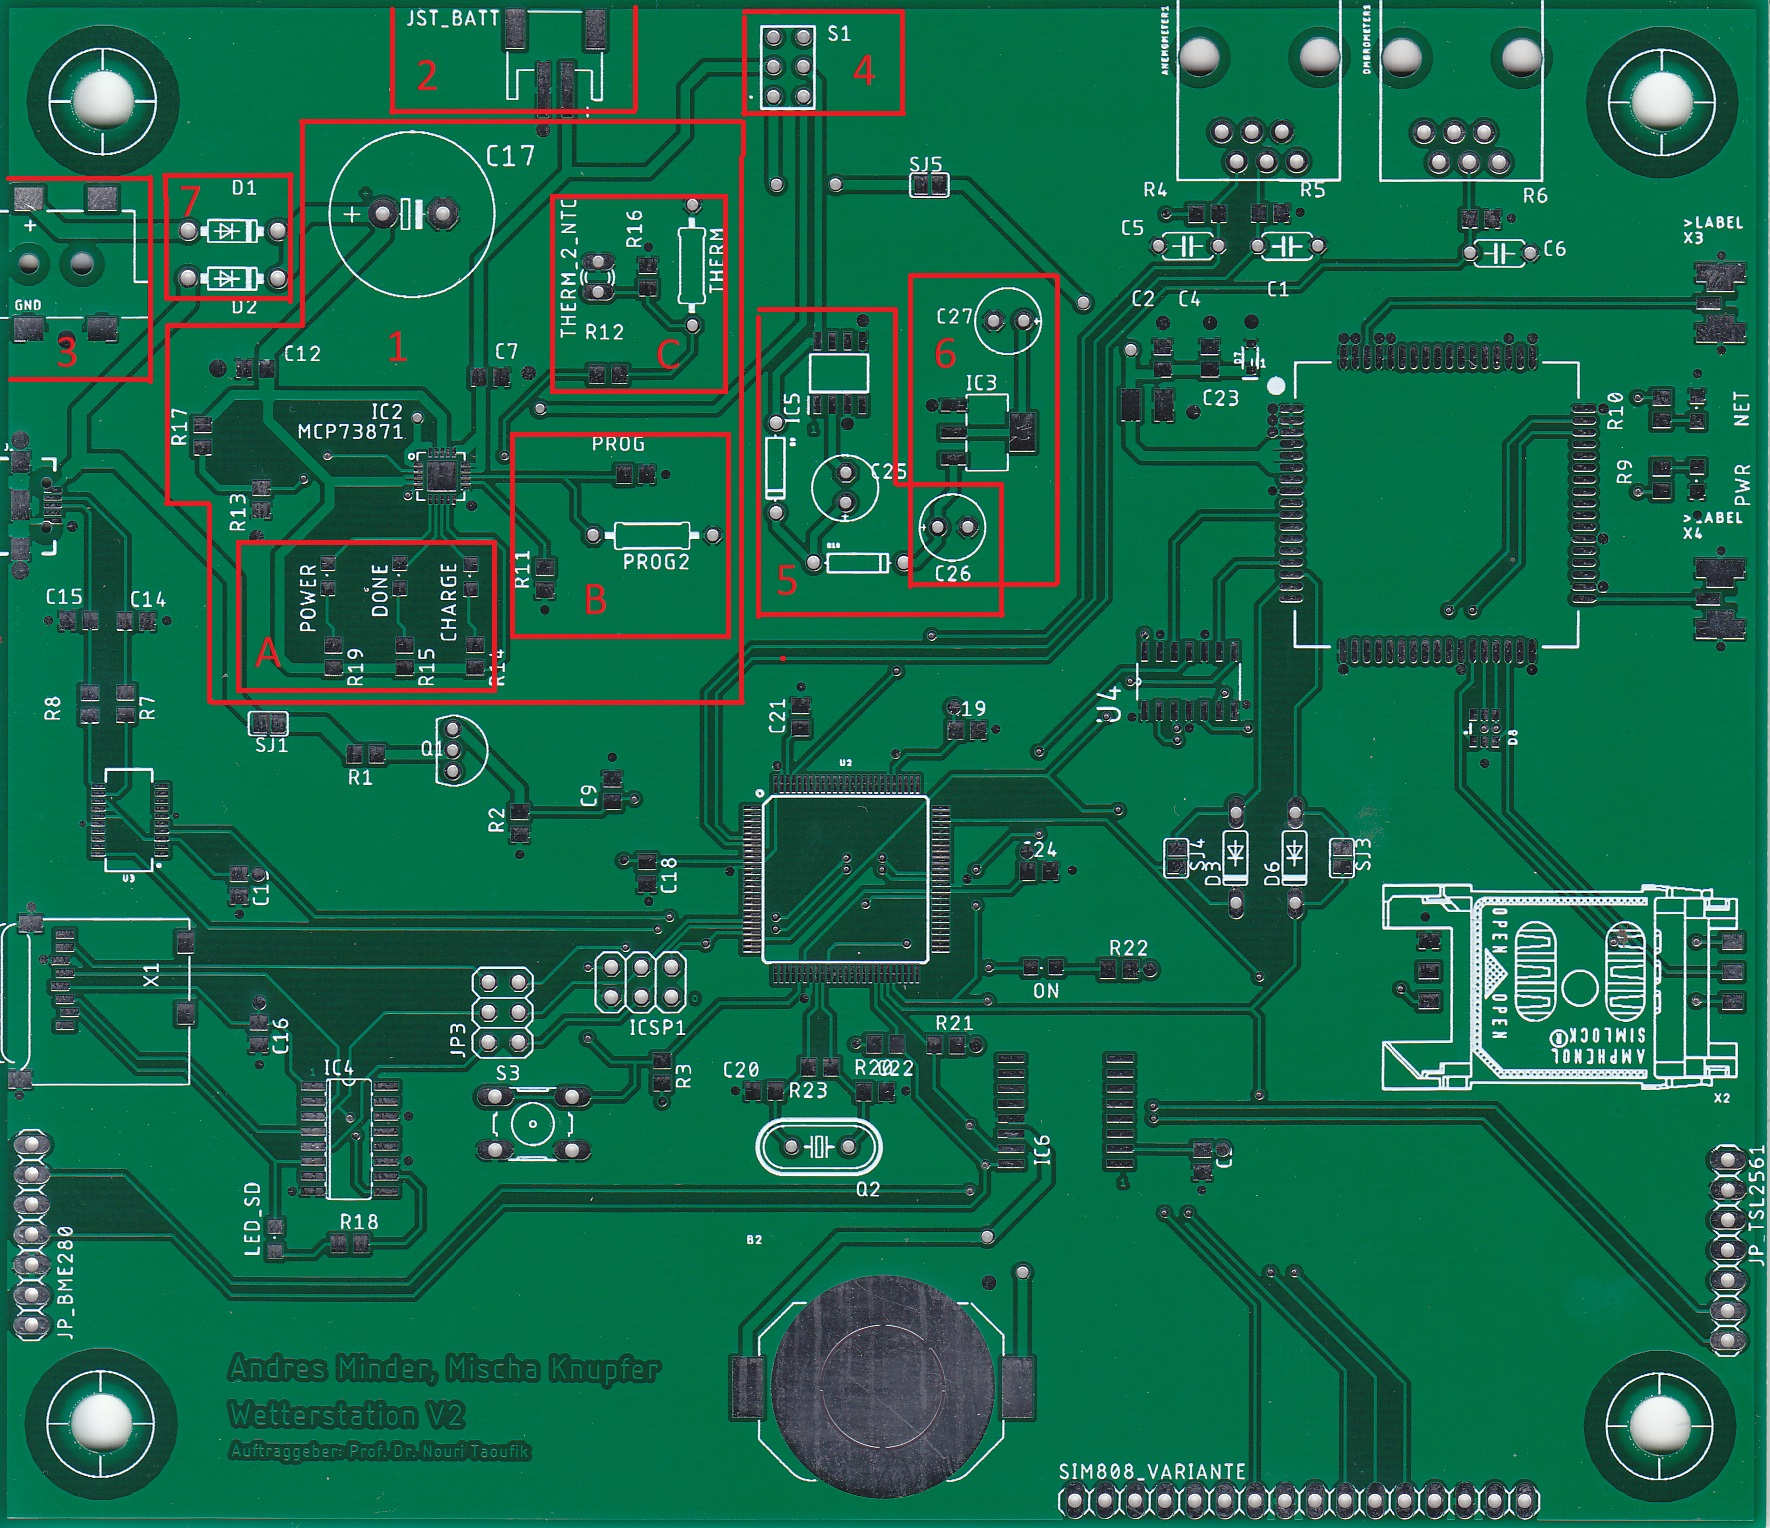
\includegraphics[width=0.99\linewidth]{graphics/HW_Uebersicht/PCB_Energieversorgung.jpg}
\caption{Das unbestückte PCB mit den markierten Bereichen für die Energieversorgung.}
\label{fig:Uebersicht_PCB_Energie}
\end{figure}
Die gesamte Schaltung für die Energieversorgung wurde in Abbildung \ref{fig:Uebersicht_PCB_Energie} in Bereiche unterteilt. Bereich 1 zeigt den MCP73871, den Power-Management-Chip, mit seinen Status-LED (1-A), sowie dessen Beschaltungen zur Einstellung des maximalen Ladestroms (1-B) und der Ausschalttemperatur (1-C). Der Anschluss für die Batterie erfolgt über den JST-Stecker (2). Über ein DC-Power Jack (3) wird die Photovoltaikanlage an die Wetterstation angeschlossen. Durch ein Schalter (4) können alle anderen Systeme der Wetterstation von der Energieversorgung getrennt werden. Die Charge-Pump (5) erhöht die erhaltene Batteriespannung, damit der Linearregler (6) die 3.3V-Ausgangsspannung mit möglichst kleinem Rippel erzeugen kann. Zwei Dioden (7) schützen die Eingänge vor rückfliessenden Strömen, indem diese nur in die gewünschte Richtung durchlassen und in die andere Richtung sperren.

In diesem Kapitel wurden die Bereiche des noch unbestückten PCBs erläutert und dadurch eine Übersicht über die Komponenten gegeben. In den nächsten Kapiteln soll auf diese Komponenten eingegangen werden, wobei mit der MCU begonnen wird.\\